\ifdefined\pdfminorversion
  \pdfminorversion=7
\fi
\documentclass[12pt,a4paper,oneside]{report}

\usepackage[margin=1in,headheight=22pt,headsep=0.28in]{geometry}
\usepackage[T1]{fontenc}
\usepackage[utf8]{inputenc}
\usepackage{helvet}
\renewcommand{\familydefault}{\sfdefault}
\usepackage{setspace}
\setstretch{1.15}
\usepackage{microtype}
\usepackage{booktabs}
\usepackage{array}
\usepackage{longtable}
\usepackage{enumitem}
\usepackage[table]{xcolor}
\usepackage{hyperref}
\usepackage{listings}
\usepackage{amsmath}
\usepackage{amssymb}
\usepackage{graphicx}
\usepackage{float}
\usepackage{caption}
\usepackage{needspace}
\usepackage{fancyhdr}
\usepackage{titlesec}
\usepackage{chngcntr}
\usepackage{tocloft}
\usepackage{etoolbox}

\definecolor{covergreen}{RGB}{35,107,72}
\definecolor{accentgreen}{RGB}{224,239,228}
\definecolor{warningyellow}{RGB}{252,244,210}

\hypersetup{
  colorlinks=true,
  linkcolor=black,
  citecolor=black,
  urlcolor=black,
  plainpages=false,
  hypertexnames=false,
  pdftitle={Accelera Auto Preprocessing, Reporting, and Benchmarking Modules},
  pdfauthor={Individual Work Draft}
}

\titleformat{\chapter}[hang]
  {\normalfont\bfseries\fontsize{24}{29}\selectfont\raggedright}
  {\chaptername\ \thechapter:}{0.5em}{}
\titleformat{name=\chapter,numberless}[hang]
  {\normalfont\bfseries\fontsize{24}{29}\selectfont}{}{0pt}{}
\titlespacing*{\chapter}{0pt}{0pt}{18pt}
\titleformat{\section}
  {\normalfont\bfseries\fontsize{18}{22}\selectfont}
  {\thesection}{0.6em}{}
\titlespacing*{\section}{0pt}{17pt}{8pt}
\titleformat{\subsection}
  {\normalfont\bfseries\fontsize{14}{18}\selectfont}
  {\thesubsection}{0.6em}{}
\titlespacing*{\subsection}{0pt}{13pt}{6pt}
\titleformat{\subsubsection}
  {\normalfont\bfseries\fontsize{12}{15}\selectfont}
  {\thesubsubsection}{0.6em}{}

\pagestyle{fancy}
\fancyhf{}
\fancyhead[R]{\textbf{Accelera} \textcolor{covergreen}{2026}}
\fancyfoot[R]{\thepage\,|\,Page}
\renewcommand{\headrulewidth}{0.5pt}
\renewcommand{\footrulewidth}{0.3pt}
\fancypagestyle{plain}{\pagestyle{fancy}}

\counterwithin{figure}{chapter}
\counterwithin{table}{chapter}
\renewcommand{\lstlistingname}{Algorithm}
\renewcommand{\lstlistlistingname}{List of Algorithms}
\setlength{\emergencystretch}{2em}
\raggedbottom
\renewcommand{\topfraction}{0.9}
\renewcommand{\bottomfraction}{0.8}
\renewcommand{\textfraction}{0.07}
\renewcommand{\floatpagefraction}{0.8}
\setcounter{tocdepth}{3}
\setcounter{secnumdepth}{3}
\renewcommand{\contentsname}{Table of Contents}
\renewcommand{\listfigurename}{List of Figures}
\renewcommand{\listtablename}{List of Tables}

\lstdefinestyle{pythonstyle}{
  language=Python,
  basicstyle=\ttfamily\small,
  keywordstyle=\color{blue!60!black},
  commentstyle=\color{green!40!black},
  stringstyle=\color{red!55!black},
  frame=single,
  breaklines=true,
  columns=fullflexible,
  keepspaces=true,
  showstringspaces=false
}

\lstdefinestyle{code}{
  basicstyle=\ttfamily\footnotesize,
  breaklines=true,
  frame=single,
  columns=fullflexible,
  keepspaces=true,
  showstringspaces=false,
  keywordstyle=\color{blue!60!black},
  commentstyle=\color{green!40!black},
  stringstyle=\color{red!50!black}
}

\lstdefinestyle{algostyle}{
  basicstyle=\ttfamily\footnotesize,
  backgroundcolor=\color{white},
  frame=tb,
  rulecolor=\color{black},
  framerule=0.45pt,
  framesep=4pt,
  breaklines=true,
  breakatwhitespace=false,
  breakautoindent=false,
  breakindent=0pt,
  columns=fullflexible,
  keepspaces=true,
  showstringspaces=false,
  captionpos=t,
  aboveskip=0.8em,
  belowskip=0.8em
}
\DeclareRobustCommand{\modulepath}[1]{\path{#1}}
\newcommand{\project}{Accelera}
\newcommand{\bestcell}{\cellcolor{accentgreen}}
\newcommand{\warncell}{\cellcolor{warningyellow}}

\begin{document}
\begin{titlepage}
\thispagestyle{empty}


\vspace*{0.5cm}

% Cairo University logo

\includegraphics[width=0.12\textwidth]{../imgs/CU_logo.png}\\\\
{\fontsize{12}{14}\selectfont Cairo University}\\
{\fontsize{12}{14}\selectfont Faculty of Engineering}\\
{\fontsize{12}{14}\selectfont Department of Computer Engineering}\\

\centering
{\bfseries\fontsize{24}{28}\selectfont Accelera}

\vspace{1.0cm}


\includegraphics[width=0.2\textwidth]{../imgs/accelera.png}

\vspace{0.4cm}

{\fontsize{12}{14}\selectfont
A Graduation Project Report Submitted\\
to\\[0.15cm]
Faculty of Engineering, Cairo University\\[0.15cm]
in Partial Fulfillment of the Requirements for the Degree\\[0.15cm]
of\\[0.15cm]
Bachelor of Science in Computer Engineering.
}
\vspace{1.0cm}

{\bfseries\fontsize{16}{14}\selectfont Presented by}

\vspace{0.3cm}

{\fontsize{14}{16}\selectfont
\begin{tabular}{>{\centering\arraybackslash}p{0.35\textwidth}>{\centering\arraybackslash}p{0.35\textwidth}}
 Nesma Osama \\ 9220912
\end{tabular}
}
\vspace{0.8cm}

{\bfseries\fontsize{16}{14}\selectfont Supervised by}

\vspace{0.2cm}

{\fontsize{14}{14}\selectfont Dr. Salma Abdel Monem}

\vspace{0.3cm}

{\fontsize{12}{14}\selectfont April 17, 2026}

\vfill

{\fontsize{11}{14}\selectfont
All rights reserved. This report may not be reproduced in whole or in part,
by photocopying or other means, without the permission of the authors or department.
}

\end{titlepage}

\pagenumbering{arabic}
\setcounter{page}{2}

\chapter*{Abstract}
\addcontentsline{toc}{chapter}{Abstract}
This report explains my individual work in three parts of the Accelera
project. The first part is Auto Preprocessing, which prepares tabular, text,
and image datasets before model training. The second part is the Accelera
Pipeline reporting part, which generates reports for pipeline graphs, branches,
and metrics. The third part is the Benchmarking module, which allows prediction
submissions to be compared using the same dataset and evaluation metric.
In this report, I describe the main idea, the steps I
followed, the generated reports, the benchmark workflow, and the testing
results.

\clearpage

\clearpage
\phantomsection
\addcontentsline{toc}{chapter}{Table of Contents}
\tableofcontents

\clearpage
\phantomsection
\addcontentsline{toc}{chapter}{List of Figures}
\listoffigures

\clearpage
\phantomsection
\addcontentsline{toc}{chapter}{List of Tables}
\listoftables

\clearpage
\phantomsection
\addcontentsline{toc}{chapter}{List of Algorithms}
\lstlistoflistings

\clearpage

\chapter*{List of Abbreviations}
\addcontentsline{toc}{chapter}{List of Abbreviations}
\begin{tabular}{ll}
AI & Artificial Intelligence \\
CSV & Comma-Separated Values \\
EDA & Exploratory Data Analysis \\
HTML & HyperText Markup Language \\
JSON & JavaScript Object Notation \\
KNN & K-Nearest Neighbors \\
ML & Machine Learning \\
NLP & Natural Language Processing \\
PDF & Portable Document Format \\
TF-IDF & Term Frequency-Inverse Document Frequency \\
UI & User Interface \\
\end{tabular}



\chapter{Introduction}
\label{chap:introduction}

\section{Motivation and Justification}
In many machine learning projects, building the model is not the only important step. Before training the model, the dataset usually needs many preparation steps such as cleaning, checking missing values, splitting the data, encoding categorical columns, scaling numerical values, and making sure there are no errors. These steps are repeated in most projects, so doing them manually every time can take a lot of time and may lead to mistakes.\\

\noindent Accelera tries to make these steps easier by providing them in one framework. The Auto Preprocessing module is responsible for preparing the data automatically. It applies the needed preprocessing steps and saves the fitted objects, such as encoders and scalers, so the same steps can be used later on new data. This is important because using different preprocessing steps between training and testing can give wrong results.\\

\noindent The Reporting in Pipeline module helps the user understand the pipeline results in a clearer way. It shows the generated graphs, explains the different branches, and allows the user to compare the results of these branches. Instead of only displaying numbers in the terminal, the module creates HTML reports that include graphs, tables, and metric summaries.\\

\noindent The Benchmarking module is used when different users want to compare their results on the same task. The benchmark creator prepares the test data and keeps the correct target values hidden. Then, users submit their predictions, and the system evaluates them using the same metric. This makes the comparison fair because all submissions are tested using the same rules.\\

\noindent These modules help reduce manual work, make the machine learning process more organized, and give users clearer results.\\

\section{Project Objectives and Problem Definition}

In machine learning projects, preparing the data and understanding the results are important steps before and after model training. However, these steps may become difficult when they are done manually, especially when the dataset contains different types of data or when the user needs to repeat the same process many times.\\

\noindent This project focuses on improving these steps inside Accelera. It aims to support the user during data preprocessing, pipeline reporting, and benchmarking. The Auto Preprocessing module prepares different types of datasets for machine learning tasks. The Reporting in Pipeline module presents the pipeline outputs in a clear form using reports, graphs, tables, and metric summaries. The Benchmarking module gives users a fair way to submit their predictions and compare their results using the same evaluation rules.\\

\noindent the main objective of this work is to make the machine learning workflow more organized, easier to understand, and less dependent on manual steps.\\


\section{Project Outcomes}
The implemented work produces three main outcomes. First, the Auto Preprocessing module prepares tabular, text, and image datasets and saves the fitted artifacts needed for later testing. Second, the reporting code generates readable preprocessing and pipeline outputs using HTML pages, tables, graphs, and metric summaries. Third, the Benchmarking module supports benchmark creation, submission validation, scoring, and leaderboard display.

\section{Document Organization}
Chapter 2 summarizes the related concepts and previous work. Chapter 3 explains the system design and architecture of Auto Preprocessing, Pipeline Reporting, and Benchmarking. Chapter 4 presents testing and comparative evaluation. Chapter 5 concludes the report and lists future improvements. The user guide is in the appendix.


\chapter{Literature Survey}
In this chapter, I give an overview of the topics, algorithms, and techniques needed to understand my work in the project. I discuss the technical subjects and background knowledge.
\section{Background and Previous Work}
This section explains the concepts and techniques used.
\subsection{Data Science}
Data science is a field that extracts knowledge and insights from data using
scientific methods, processes, and algorithms.
\subsection{ML}
Machine learning is a field of artificial intelligence that lets computers learn patterns from data without needing to be explicitly programmed. 
A machine learning model is trained using training data , and then it uses what it learned to make predictions on new data.

\subsection{Supervised ML}
The training dataset includes a label column that represents the target output. 
This column is used during training to learn the mapping between the input features and the expected result.
\subsection{Classification}
Classification is a supervised machine learning task whose output is a label or category.

\subsection{Regression}
Regression is a supervised machine learning task whose output is a continuous numerical value.
\subsection{NLP}
Natural language processing is a field that focuses on enabling computers to understand and work with human language. Text data can't be used directly by most machine learning models, so it needs to be cleaned and turned into numerical features first.

\subsection{EDA}
Exploratory Data Analysis is an important step in data analysis where we explore,
summarize, and visualize data to understand its structure, detect patterns, 
and check relationships between variables.

\subsection{Data Preprocessing}
Data preprocessing is the stage of transforming raw data into a clean and usable
format for machine learning models.


\subsection{Missing Value Imputation}
Missing value imputation is a preprocessing technique used when some values in a
dataset are empty. Instead of removing all rows that contain missing
values, the missing values can be replaced using a suitable value.

\subsection{Robust Scaling}
Robust scaling is a scaling technique that uses the median and the
interquartile range instead of the mean and standard deviation. 
\[
x' = \frac{x - \mathop{\mathrm{median}}(X)}{\mathop{\mathrm{IQR}}(X)}
\]
where $x'$ is the scaled value, $x$ is the original value,
$\mathop{\mathrm{median}}(X)$ is the median of the feature values, and
$\mathop{\mathrm{IQR}}(X)$ is the interquartile range.
\subsection{Categorical Encoding}
Categorical encoding is the process of converting text categories into numeric
values. Many traditional machine learning models and preprocessing pipelines
expect numerical input.

\subsection{Binary Encoding}
Binary encoding is a categorical encoding technique that first gives each
category a number, then converts this number into binary form. The binary digits
are then stored as separate columns. 

\subsection{Frequency Encoding}
Frequency encoding replaces each category with how often it appears in the
dataset. If a category appears many times, it receives a higher frequency value.
\[
f(c) = \frac{\mathop{\mathrm{count}}(c)}{N}
\]
where $f(c)$ is the frequency of category $c$,
$\mathop{\mathrm{count}}(c)$ is the number of rows containing this category,
and $N$ is the total number of rows.

\subsection{TF-IDF}
It is a technique used to convert text into numerical features by giving each word a weight based
on how important it is in a document and across the whole dataset.
Term Frequency measures how often a word appears in a document. Inverse Document
Frequency gives lower weight to words that appear in many documents, because
these words are usually less useful for classification.
\[
TFIDF(t,d) = TF(t,d) \times IDF(t)
\]
where $TFIDF(t,d)$ is the weight of term $t$ in document $d$, $TF(t,d)$ is the
frequency of the term in the document, and $IDF(t)$ measures how rare the term
is across all documents.
\subsection{Data augmentation}
Is a technique used to increase diversity of a dataset without actually collecting new data. 
It works by applying various transformations to the existing data to create new, modified versions of data that helps the model generalize better.
\subsection{Classification Evaluation Metrics}
Classification metrics are used to evaluate the performance of a classification
model.
\subsubsection{Accuracy}
Accuracy measures how many predictions are correct out of all predictions:
\[
Accuracy = \frac{TP + TN}{TP + TN + FP + FN}
\]
where $TP$ is true positives, $TN$ is true negatives, $FP$ is false positives,
and $FN$ is false negatives.
\subsubsection{Precision}
Precision measures how many predicted positive samples are actually positive:
\[
Precision = \frac{TP}{TP + FP}
\]
\subsubsection{Recall}
Recall measures how many actual positive samples were correctly detected:
\[
Recall = \frac{TP}{TP + FN}
\]
\subsubsection{F1-score}
The F1-score combines precision and recall:
\[
F1 = 2 \times \frac{Precision \times Recall}{Precision + Recall}
\]


\subsection{Regression Evaluation Metrics}
Regression metrics are used when the model predicts continuous numerical values.
\subsubsection{Mean Absolute Error}
Mean Absolute Error measures the average absolute difference between the real
values and predicted values:
\[
MAE = \frac{1}{n}\sum_{i=1}^{n}|y_i - \hat{y}_i|
\]
where $y_i$ is the actual value and $\hat{y}_i$ is the predicted value.
\subsubsection{Mean Squared Error}
Mean Squared Error gives more penalty to large errors:
\[
MSE = \frac{1}{n}\sum_{i=1}^{n}(y_i - \hat{y}_i)^2
\]
\subsubsection{R-squared Score}

R-squared score measures how well the regression model explains the variation in the actual values. 
\[
R^2 = 1 - \frac{\sum_{i=1}^{n}(y_i - \hat{y}i)^2}{\sum_{i=1}^{n}(y_i - \bar{y})^2}
\]
Where $y_i$ is the actual value, $\hat{y}_i$ is the predicted value, and $\bar{y}$ is the mean of the actual values.



\section{Comparative Study of Previous Work}
The most direct external comparison in this report is AutoCleanML because it also automates common tabular preprocessing tasks. The comparison focuses on the effect of preprocessing on model results, using the same validation split and the same machine learning models where possible.

\section{Implemented Approach}

\subsection{Auto Preprocessing}
In this module I decided to implement an automated preprocessing approach for tabular datasets. The
approach was designed to prepare data for machine learning models by applying
suitable preprocessing steps automatically according to the type and
characteristics of each column and some user configurations.

\noindent The general framework of the approach is as follows:
\begin{enumerate}
  \item Take the dataset and some user configurations.
  \item Remove duplicate records.
  \item Split the data into training and validation sets.
  \item For each column, we get this information: data type, percentage of missing values, unique values, and basic stats.
  \item Drop unnecessary columns, such as constant columns or columns with
  missing values above the selected threshold.
  \item Detect column types automatically.
  \item Make Exploratory Data Analysis.
  \item Apply missing value imputation.
  \item Apply categorical encoding.
  \item Apply robust scaling.
  \item Apply feature selection using mutual information.
  \item Automatically saves all needed files for inference.
  \item Generate a report.
\end{enumerate}

\noindent The chosen approach follows a classical automated preprocessing pipeline. The
main preprocessing decisions are:

\begin{itemize}
  \item \textbf{Missing values:} Median imputation is used for numerical
  features because it is simple and more robust to outliers than mean
  imputation. For categorical features, most-frequent imputation is used because
  it replaces missing values with valid existing categories.

  \item \textbf{Numerical scaling:} \texttt{RobustScaler} is used for numerical
  features because tabular datasets may contain outliers or skewed values. It
  depends on the median and interquartile range, which makes it more stable than
  standard scaling when extreme values exist.

  \item \textbf{Categorical encoding:} The encoding method is selected according
  to the feature type and cardinality. Binary columns are encoded using ordinal
  encoding, low-cardinality categorical columns are encoded using binary
  encoding, and high-cardinality categorical columns are encoded using frequency
  encoding. This helps reduce the number of generated features and avoids high
  dimensionality.

  \item \textbf{Feature selection:} Mutual information is used because it is a
  filter-based method that can work with both classification and regression
  tasks. It helps keep the most informative features and remove weak features
  before model training.
\end{itemize}

\noindent This approach was chosen because it gives a good balance between automation,
simplicity, and speed. More advanced techniques, such as
K-nearest neighbour imputation, autoencoders, and wrapper feature selection, can
be useful in specific cases, but they need more computation.

\noindent One of the important additions in this project is that the module is not
only used for data preparation. It also supports exploratory data analysis report.

\noindent Also the module was extended to support text and image data
preparation, not only tabular data.
\subsection{Reporting in Pipeline}

In this Part of the module, I implemented a simple reporting approach to help the user
understand the pipeline results. Sometimes the pipeline produces many outputs,
such as graphs,  and different branch results. If these results
are only shown in the terminal, they may be difficult to read and compare.

\noindent The general framework of the approach is as follows:
\begin{enumerate}
  \item Take the results produced by the pipeline.
  \item Take the graph from XML file.
  \item Collect the metric results for each branch.
  \item Put all the information in an organized HTML report.
\end{enumerate}

\noindent The main idea of this module is to make the pipeline output easier to
read. The report shows the important results in one place instead of leaving the
user to search through terminal outputs or many files.

\noindent The main reporting parts are:

\begin{itemize}
  \item \textbf{Pipeline graph:} The report first shows the full pipeline graph.
  This graph helps the user understand the general structure of the pipeline and
  how the branches are connected.

  \item \textbf{Branch nodes:} After that, the report shows the nodes inside each
  branch. This helps the user understand the steps that were applied in every
  branch separately.

  \item \textbf{Branch comparison:} By showing the metric results for all
  branches together, the report helps the user compare the branches and see
  which one performed better.
\end{itemize}

\noindent This approach was chosen because it makes the results clearer and easier
to review. It also separates the reporting part from the main pipeline logic,
which makes the system more organized.

\subsection{Benchmarking}

In this module, I implemented a benchmarking approach to compare machine
learning submissions in a fair way. The module allows users to submit their
prediction files and evaluates all submissions using the same test data, target
values, and metric. This makes the comparison fair because all users are tested
under the same conditions.

\noindent The module also supports learning between users. After submissions are
evaluated, users can view other users' code and results. This helps them
understand different solution ideas, learn from stronger submissions, and improve
their own work in future trials.



\noindent The general framework of the approach is as follows:
\begin{enumerate}
  \item Create a benchmark task.
  \item Separate the test data from the correct target values.
  \item Allow users to submit their prediction files.
  \item Check the submitted file format.
  \item Compare the submitted predictions with the correct target values.
  \item Calculate the score using the selected metric.
  \item Show the results in a leaderboard.
\end{enumerate}

\noindent The main idea of this module is to keep the evaluation fair. All users are
tested using the same test data, the same target file, and the same metric.

\noindent The main benchmarking parts are:

\begin{itemize}
  \item \textbf{Hidden target values:} The correct answers are kept hidden from
  the users to make the comparison fair.

  \item \textbf{Prediction submission:} Users only submit their predicted values.

  \item \textbf{Metric evaluation:} The system calculates the score using the
  selected evaluation metric.

  \item \textbf{Leaderboard:} The results are displayed in a leaderboard so users
  can compare their scores easily.
\end{itemize}

\noindent This approach was chosen because it gives a simple and fair way to compare
different machine learning solutions. It also reduces manual checking and makes
the evaluation process automatic.

\chapter{System Design and Architecture}
\label{chap:system-design}
This chapter explains the design of the modules included in this individual report. The main modules are Auto Preprocessing, Accelera Pipeline Reporting, and the Benchmarking Platform.
\section{Overview and Assumptions}
The design of these modules depends on some assumptions.
\subsection{Auto Preprocessing Assumptions}

For the Auto Preprocessing module, the assumptions depend on the type of dataset being processed. The module supports three types of data: tabular, text, and image datasets.

\subsubsection{Tabular Dataset Assumptions}

For tabular datasets, the Auto Preprocessing module assumes that:

\begin{itemize}
\item The dataset consists of numerical and categorical features, and the task is either classification or regression.  
Because we try to implement the standard structured machine learning problems where supervised learning is applied..
\item The user provides configuration parameters to control preprocessing operations.  
This allows the pipeline to adapt to different datasets and user requirements.
\end{itemize}
\subsubsection{Text Dataset Assumptions}

For text datasets, the Auto Preprocessing module assumes that:

\begin{itemize}
\item we assume that the dataset has one text column and one categorical target label.This makes the pipeline easier to apply and keeps the number of features smaller after converting the text into numerical values.
\item The user provides configuration parameters for text cleaning and feature extraction.  
To give the user a level of control over the preprocessing pipeline.
\end{itemize}

\subsubsection{Image Dataset Assumptions}
\begin{itemize}

\item The dataset is for image classification and follows this folder structure.  
\begin{verbatim}
Training/
  Cats/
  Dogs/

Validation/
  Cats/
  Dogs/
\end{verbatim}
\item All images are stored in supported formats and are accessible.  
This ensures compatibility with image loading and preprocessing libraries.

\item The user provides configuration parameters for preprocessing and augmentation.  
Because different datasets require different preprocessing strategies such as resizing, normalization, and augmentation.

\end{itemize}

\subsection{Benchmark Assumptions}

For the Benchmark module, the following assumptions are made. These assumptions are introduced due to system design constraints, particularly the limited server storage capacity for handling large dataset uploads.

\begin{itemize}

\item When the user creates a benchmark, they provide a tabular dataset. This ensures that the module operates on structured data suitable for standard machine learning evaluation.

\item All datasets are stored in publicly accessible Google Drive links. This design choice is adopted to reduce server storage requirements.

\item The user must provide three CSV files:
\begin{itemize}
\item A training dataset containing both features and target labels.
\item A testing dataset containing the same feature structure as the training set but without the target column.
\item A ground truth target file containing only the target labels for the test set.
\end{itemize}
This separation ensures a standard evaluation protocol and prevents data leakage during benchmarking.

\item When submitting predictions, the user provides a Google Drive link to a CSV file containing the predicted results. This ensures consistency in submission format across all users.

\item The submitted prediction file must have the same length and format as the expected output to ensure correct evaluation and fair comparison between different users' models.

\item When creating a benchmark, it is assumed that the user selects an evaluation metric that is appropriate for the problem type and provides a correct metric configuration. This is necessary to guarantee meaningful and valid performance measurement.

\item For admin users, when defining an evaluation metric, it is assumed that a valid metric from the Scikit-learn library is selected. Because we use Scikit-learn metrics for evaluation.
\item The selected metric must be properly configured and is expected to return a single scalar value for performance comparison and ranking purposes.

\item The user is allowed to have only one active submission per benchmark. The user cannot create multiple submissions, but they are allowed to update their existing submission. This constraint is enforced to reduce storage usage.

\end{itemize}
\subsection{Reporting Module Assumptions}
 
The Reporting in Pipeline module depends on the following assumptions:

\begin{itemize}
  \item The metric results are already generated from the pipeline modules.

  \item The metric result should be one of the supported types, such as a number,
  array, dictionary, string, or tuple.

  \item If the metric result needs to be displayed as a figure, the user should
  provide a plotting function.
  \item Figures are supported only in specific cases. If the metric result is a
multi dimensional array or tuple and the user wants to display it as a graph, the user should provide a plotting function.
  \item The plotting function should take the metric result as input and return
  the correct Matplotlib \texttt{plt} object.

  \item The output folder path should be valid so the generated report and images
  can be saved.
\end{itemize}


\section{System Architecture}

This section explains the implemented modules in this report. It discusses the three main parts: Auto Preprocessing, Pipeline Reporting, and Benchmarking. For each module, the section explains module overview and how it works.
\section{Auto Preprocessing Module}

\subsection{Module Overview}
The module supports three dataset families:

\begin{itemize}[leftmargin=*]
  \item tabular datasets for classification and regression;
  \item text datasets for classification; and
  \item image datasets for classification.
\end{itemize}

\noindent The workflow starts from the raw data and user configuration. The module then
applies suitable preprocessing steps and saves both the processed output and
the fitted objects required for later use. It also has its own preprocessing
reports. These reports are different from the pipeline report because they
focus on the dataset itself: data overview, missing values, duplicate rows,
column types, graphs, preprocessing decisions, selected features, and examples
of the transformed data.



\subsection{Tabular Training Flow}
\begin{figure}[!htbp]
\centering
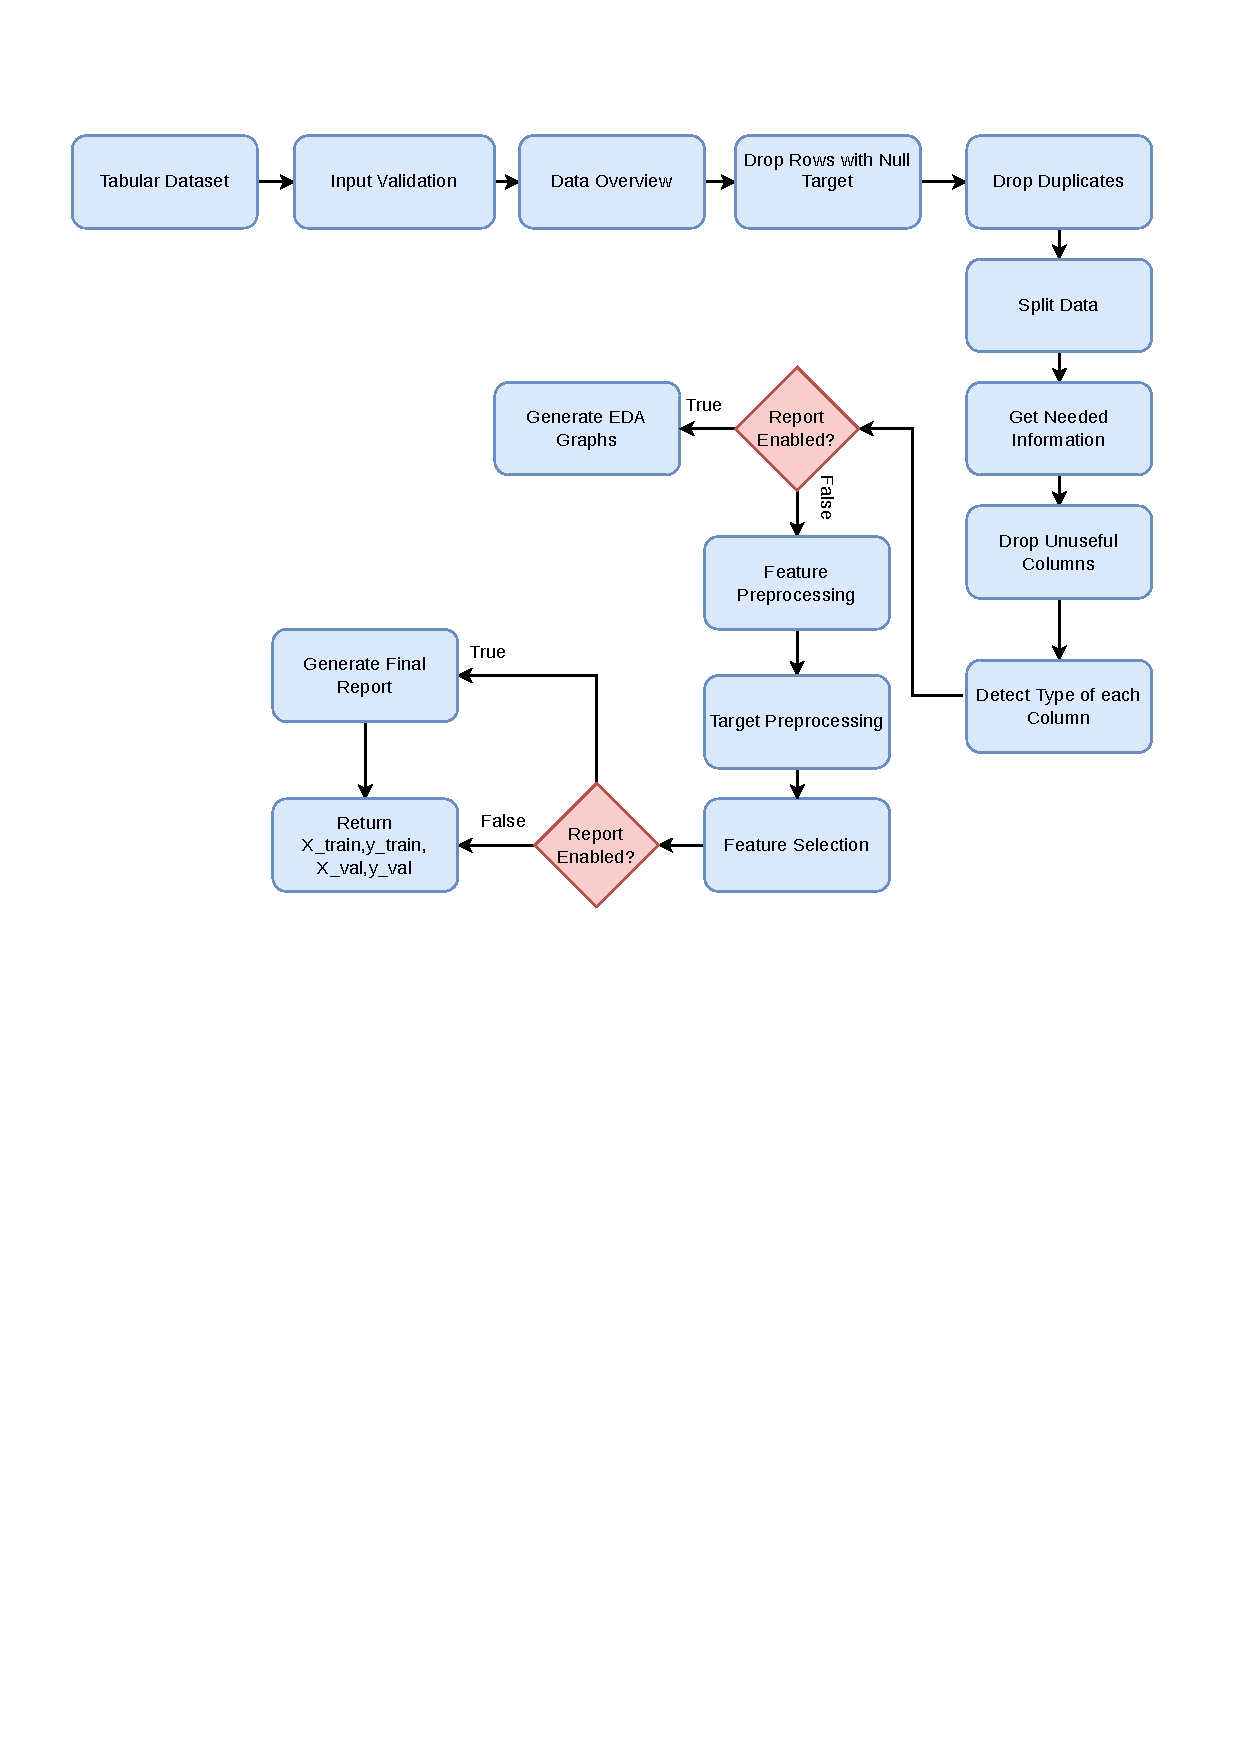
\includegraphics[width=\textwidth,trim=0mm 5mm 0mm 0mm,clip]{../imgs/tabular.pdf}
\caption{Tabular preprocessing workflow}
\label{fig:nesma-tabular-preprocessing-workflow}
\end{figure}
\noindent The tabular training flow is implemented mainly in
\modulepath{classical_training_preprocessing.py}. The class receives a pandas
DataFrame, target column, problem type, folder path, validation size, random
state, thresholds, and report flag.

\noindent The training flow starts by validating the configuration. It checks the problem
type, target column, validation size, random state, maximum ordinal threshold,
cardinality threshold, missing value threshold, and feature importance
threshold. It also saves the original input columns in
\modulepath{data_columns.pkl}, because the testing stage needs to compare new
data against the same training structure.

\noindent The training flow is:

\begin{enumerate}[leftmargin=*]
  \item validate the input configuration
  \item save original data columns for later testing
  \item create a data overview for the report
  \item remove rows has null target
  \item remove duplicate rows
  \item split data into training and validation sets
  \item detect columns that should be dropped
  \item detect each column type
  \item generate graphs if reports are enabled
  \item build a column transformer for feature preprocessing
  \item preprocess the target according to classification or regression
  \item apply feature selection using mutual information
  \item save all fitted objects and metadata 
  \item generate the HTML report.
\end{enumerate}

\begin{lstlisting}[style=algostyle,caption={General tabular preprocessing flow}]
Input: DataFrame D, target column y, problem type, other configurations
Output: X_train, X_val, y_train, y_val

1:  Validate configuration
2:  Store original dataset columns
3:  Build data overview and report information
4:  remove rows has null target
5:  Remove duplicate rows
6:  Split into training and validation sets
7:  Drop user-selected, high-missing, constant, and unsupported columns
8:  Detect column types from training data
9:  Generate feature and target graphs when report is enabled
10:  Fit feature preprocessing objects on X_train
11: Transform X_train and X_val
12: Fit target preprocessing object on y_train
13: Transform y_train and y_val
14: Select useful features using mutual information
15: Save fitted objects and metadata
16: Generate report if enabled
\end{lstlisting}

\Needspace{8\baselineskip}

\subsection{Data Overview and Cleaning}

Before applying feature transformations, the module creates a detailed data
overview .The original first rows are stored, then all string values are converted to lowercase and another preview
is stored.This helps categorical and text like values become more consistent before
splitting and encoding.\\

\noindent The overview also records dataframe information, numerical statistics,
categorical statistics, missing values per column, duplicate count, duplicate
percentage, and dataset shape. After this, rows with missing target values are
removed, because the model cannot learn correctly without a target label. Then
duplicate rows are dropped and the new shape is stored in the report data.\\

\noindent For classification tasks, the split is stratified when the target has more
than one class and contains no null values. The goal is to keep the class distribution
closer between training and validation data. For other cases, the normal
\modulepath{train_test_split} function is used with the configured
\modulepath{val_size} and \modulepath{random_state}.\\

\subsection{Tabular Column Type Detection}

The module assigns a type to each feature and then chooses preprocessing based
on the type. This rule based design is easy to understand and works without
writing special code for every dataset.\\

\noindent For every column, the module calculates the data type, number of unique values,
unique value ratio, missing value count, missing value ratio, constant value
status, mode, and for numerical columns the  minimum, maximum,
median, and mean. A feature can be dropped if the user listed it in \modulepath{columns_need_to_drop}, if it is
constant, or if its missing value ratio is greater than \modulepath{missing_threshold}.\\

\begin{table}[H]
\centering
\caption{Detected tabular column types and preprocessing}
\label{tab:column-types}
\begin{tabular}{p{0.28\textwidth}p{0.32\textwidth}p{0.30\textwidth}}
\toprule
Column type & Detection rule & Applied preprocessing \\
\midrule
Binary & columns with exactly two unique values. &
Most frequent imputation followed by ordinal encoding with unknown values
mapped to -1. \\
Ordinal & Integer columns with unique values less than or equal to
\modulepath{max_unique_ordinal}. & Most frequent imputation followed by robust
scaling. \\\\
Numerical & Integer columns with unique values greater than
\modulepath{max_unique_ordinal}. & Median imputation followed by robust
scaling. \\\\
Continuous & Floating point columns. & Median imputation followed by robust
scaling. \\
Low cardinality categorical & Object columns with unique values less than or
equal to \modulepath{cardinality_threshold}. & Most frequent imputation
followed by binary encoding. \\\\
High cardinality categorical & Object columns with unique values greater than
\modulepath{cardinality_threshold}. & Most frequent imputation followed by
frequency encoding. \\\\
Unsupported or other & Any unsupported data type. & Removed from the
preprocessing pipeline. \\
\bottomrule
\end{tabular}
\end{table}

\subsection{Tabular EDA Graphs}

The EDA part is generated per column, not as one general graph for the whole
dataset. In \modulepath{make_graphs}, the module loops over the training
feature columns after their types are detected. For each column, it chooses the
correct graph wrapper based on both the column type and the problem type. After
all feature graphs are generated, it adds a target graph and a numeric
correlation matrix.

\begin{table}[H]
\centering
\caption{EDA graphs generated for tabular preprocessing}
\label{tab:tabular-eda-graphs}
\begin{tabular}{p{0.28\textwidth}p{0.25\textwidth}p{0.37\textwidth}}
\toprule
Column type & Problem type & Generated graphs \\
\midrule
Binary and categorical & Classification & Null vs non null pie chart,
category count plot, and category count split by target class. \\
Binary and categorical & Regression & Null vs non null pie chart, category
count plot, and target box plot for each category. \\
Ordinal & Classification & Null vs non null pie chart, ordered count plot, and
ordered count plot split by target class. \\
Ordinal & Regression & Null vs non null pie chart, ordered count plot, and
target box plot for each ordinal value. \\
Numerical and continuous & Classification & Null vs non null pie chart,
histogram with KDE, and feature box plot grouped by class. \\
Numerical and continuous & Regression & Null vs non null pie chart, histogram
with KDE, and scatter plot between feature and target. \\
Target column & Classification & Null vs non null pie chart and target class
count plot. \\
Target column & Regression & Null vs non null pie chart, target histogram with
KDE, and target box plot. \\
Numeric columns & Both & Correlation heatmap. \\
\bottomrule
\end{tabular}
\end{table}

\noindent For categorical columns with many values, the graph wrappers keep the top five
categories and group the remaining values as \modulepath{Other}. This keeps the
graphs readable and avoids a very crowded x axis.

\subsection{Target Processing}

Target null rows are removed before the data split. After feature
preprocessing, the target is processed according to the problem type. For
classification, the target labels are encoded using \modulepath{LabelEncoder}.
For regression, the target values are scaled using \modulepath{RobustScaler}.
The fitted target preprocessor is saved as \modulepath{target_preprocessor.pkl},
and target metadata is saved in \modulepath{target_info.pkl}. In testing, this
metadata is used to apply the same target transformation when labels are
provided.

\subsection{Feature Selection}

After feature preprocessing, the module applies mutual information based
feature selection. For classification it uses mutual information for
classification tasks, and for regression it uses mutual information for
regression tasks. The selected features are saved in
\modulepath{selected_features.pkl}. This reduces unnecessary feature columns
and keeps the testing stage aligned with training.

\subsection{Saved Tabular Artifacts}

\begin{table}[!htbp]
\centering
\caption{Saved artifacts for tabular preprocessing}
\label{tab:tabular-artifacts}
\begin{tabular}{p{0.36\textwidth}p{0.54\textwidth}}
\toprule
Artifact & Purpose \\
\midrule
\modulepath{data_columns.pkl} & Original input columns before preprocessing. \\
\modulepath{col_drop.pkl} & Columns removed during training preprocessing. \\
\modulepath{training_preprocessor.pkl} & Fitted feature transformer. \\
\modulepath{feature_names.pkl} & Names of generated transformed features. \\
\modulepath{target_preprocessor.pkl} & Fitted label encoder or target scaler. \\
\modulepath{target_info.pkl} & Target metadata used during testing. \\
\modulepath{bool_type_col.pkl} & Boolean columns that need consistent handling. \\
\modulepath{selected_features.pkl} & Feature names selected after
mutual information. \\
\bottomrule
\end{tabular}
\end{table}

\subsection{Tabular Testing Flow}

The testing class loads the saved artifacts and applies the same
transformations to new data. The testing data must not fit a new preprocessor.
It should only use what was fitted during training.
The test data is checked against the saved column list, dropped columns are
removed, feature preprocessing is applied, selected features are kept, and the
target is transformed if it exists.

\subsection{Text Training Flow}

\begin{figure}[H]
\centering
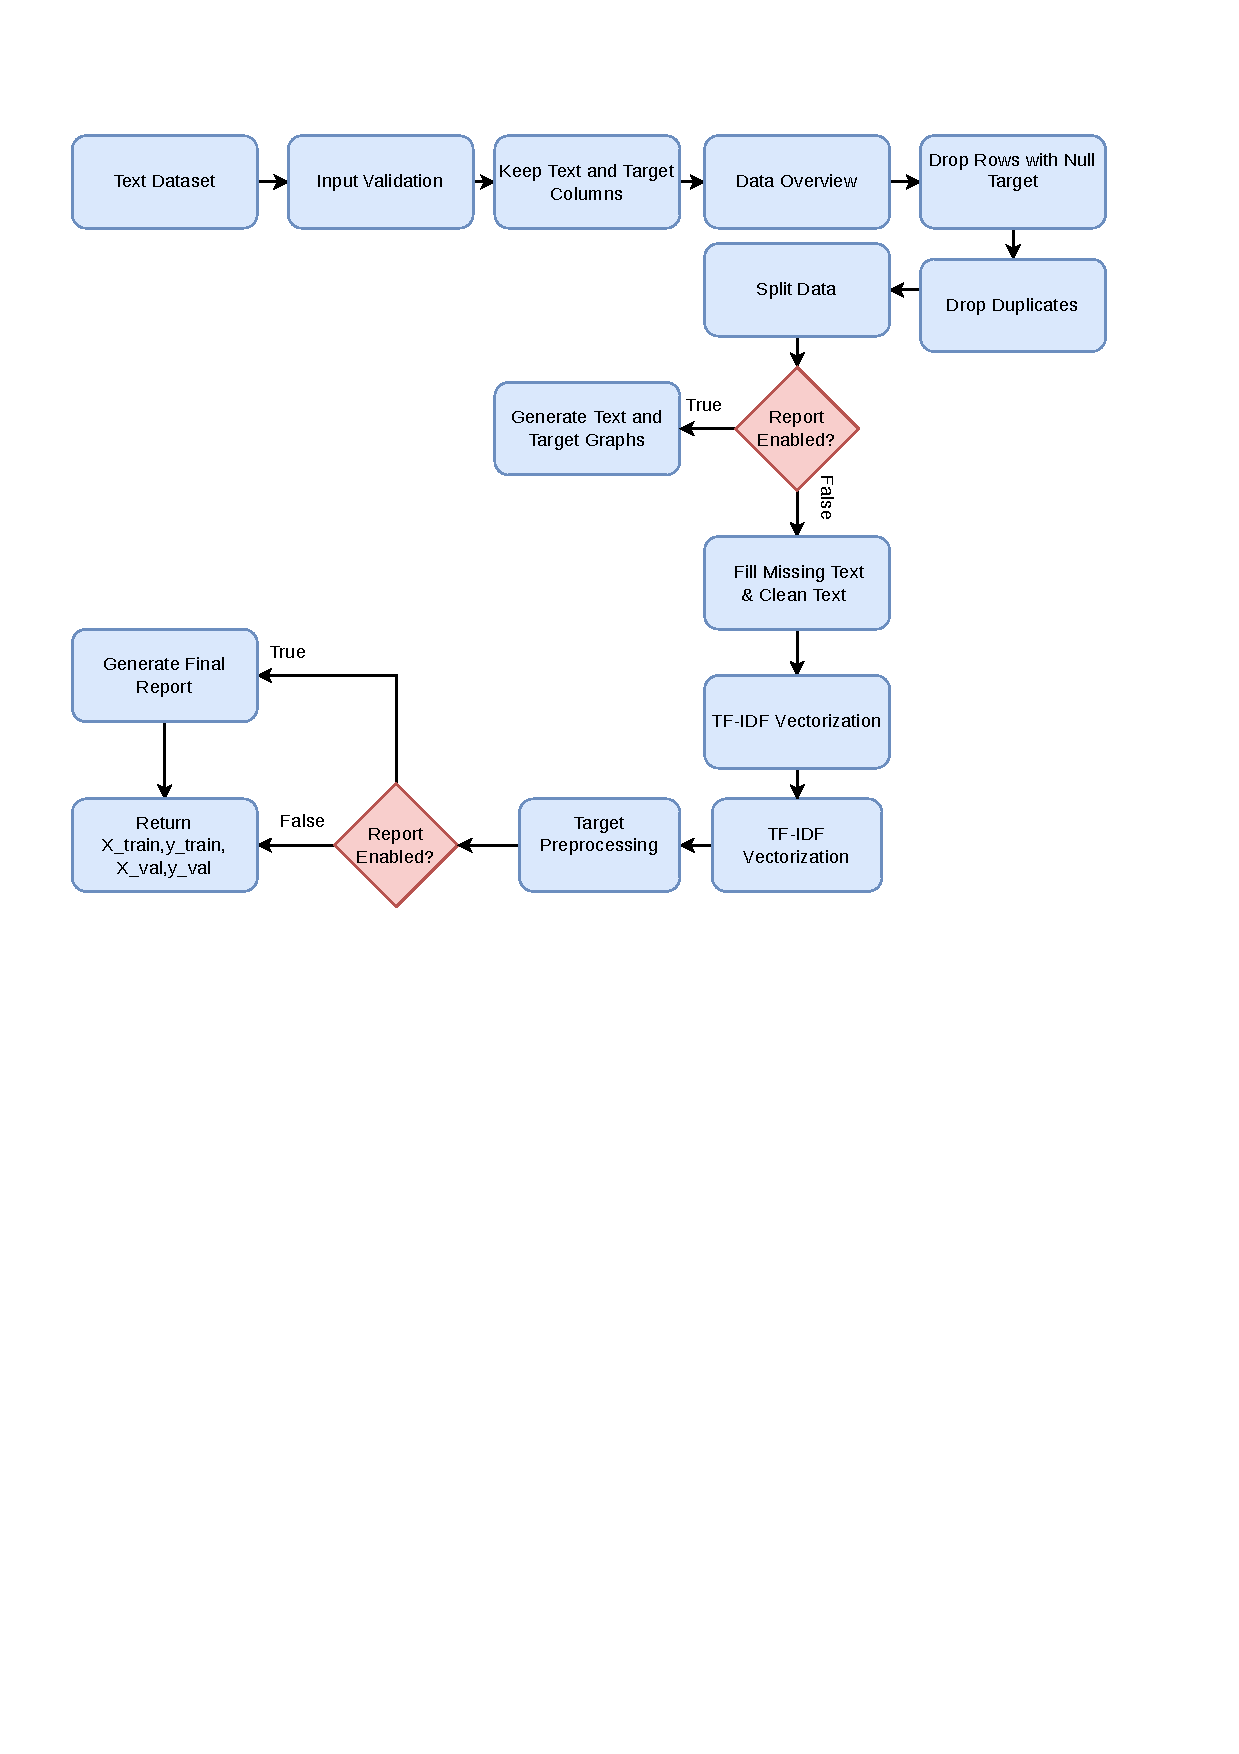
\includegraphics[width=\textwidth,trim=0mm 5mm 0mm 0mm,clip]{../imgs/text.pdf}
\caption{Text preprocessing workflow}
\label{fig:nesma-text-preprocessing-workflow}
\end{figure}


The text preprocessing class is used when the dataset contains a text column
and a target column. It inherits shared tabular behavior for overview,
duplicates, and splitting, but it uses text-specific feature preprocessing.
During initialization, the class validates that the text column exists, that it
is different from the target column, that the text column has object type, and
that the target is suitable for classification. Any columns other than the text
column and target column are removed because the text pipeline is designed for
one text feature.\\

\noindent The text flow is:

\begin{enumerate}[leftmargin=*]
  \item generate a dataset overview
  \item remove duplicate rows
  \item split into training and validation sets
  \item generate optional graphs such as target distribution and top word
        frequency
  \item fill missing text values with an empty string
  \item clean and tokenize text
  \item transform text using TF-IDF
  \item encode the target labels
  \item save TF-IDF vectorizer, label encoder, and metadata 
  \item generate the report if enabled.
\end{enumerate}

\noindent The report graphs for text are simpler than tabular column graphs. The
\modulepath{TextGraph} wrapper creates a null vs non null pie chart for the
text column and a top word frequency plot. The target graph is generated using
the classification target wrapper, so the user can also see the class
distribution. This is useful because text datasets often have missing text,
very frequent repeated words, and imbalanced labels.

\subsection{Text Tokenization}

The custom tokenizer lowercases the text, handles common contractions, keeps
important negation words such as \texttt{not} and \texttt{no}, removes noise
characters, separates digits from letters, removes short tokens, and applies
Porter stemming. This prepares the text before TF-IDF vectorization.
The fitted \modulepath{TfidfVectorizer} is saved as
\modulepath{training_preprocessor.pkl}, while the target label encoder and
metadata are saved for test-time reuse.

\noindent The tokenizer also normalizes special apostrophe characters and expands words
such as \modulepath{can't}, \modulepath{won't}, and \modulepath{shan't}. This
detail matters because negation can change the meaning of a sentence. For
example, removing the word \modulepath{not} can make a negative review look
positive, so the stopword list keeps \modulepath{not} and \modulepath{no}.

\begin{lstlisting}[style=algostyle,caption={Text tokenizer flow from the implementation}]
Input: raw text sentence
Output: cleaned token list

1:  Convert text to lowercase and remove extra spaces
2:  Normalize apostrophe characters
3:  Expand common negative contractions
4:  Add spaces between letters and digits
5:  Remove characters except letters, digits, and apostrophes
6:  Split text into words
7:  Remove stopwords except "not" and "no"
8:  Remove very short tokens
9:  Apply Porter stemming
10: Return cleaned tokens
\end{lstlisting}

After cleaning, the module fits TF-IDF on the training text only and transforms
the validation text with the same vectorizer. This avoids fitting on validation
data. The report stores a small before-and-after preview, where the original
text is shown beside the cleaned and stemmed tokens. For the target, the module
uses \modulepath{LabelEncoder} and saves it as
\modulepath{target_preprocessor.pkl}. It also saves \modulepath{data_info.pkl}
with the text column, target column, and target mode so the testing class can
reuse the same configuration.

\subsection{Text Testing Flow}

The text testing class loads \modulepath{data_info.pkl},
\modulepath{training_preprocessor.pkl}, and \modulepath{target_preprocessor.pkl}.
It checks that the test dataframe contains the saved text column. If the target
column is missing, it works in feature-only mode and returns transformed
features with no labels.

The testing flow lowercases the test data, fills missing text values with an
empty string, and applies the saved TF-IDF vectorizer. If labels exist, missing
target values are filled using the saved target mode, then transformed with the
saved label encoder. This keeps the testing behavior close to training and
prevents the test set from fitting its own vocabulary or label mapping.

\subsection{Image Training Flow}

\begin{figure}[!htbp]
\centering
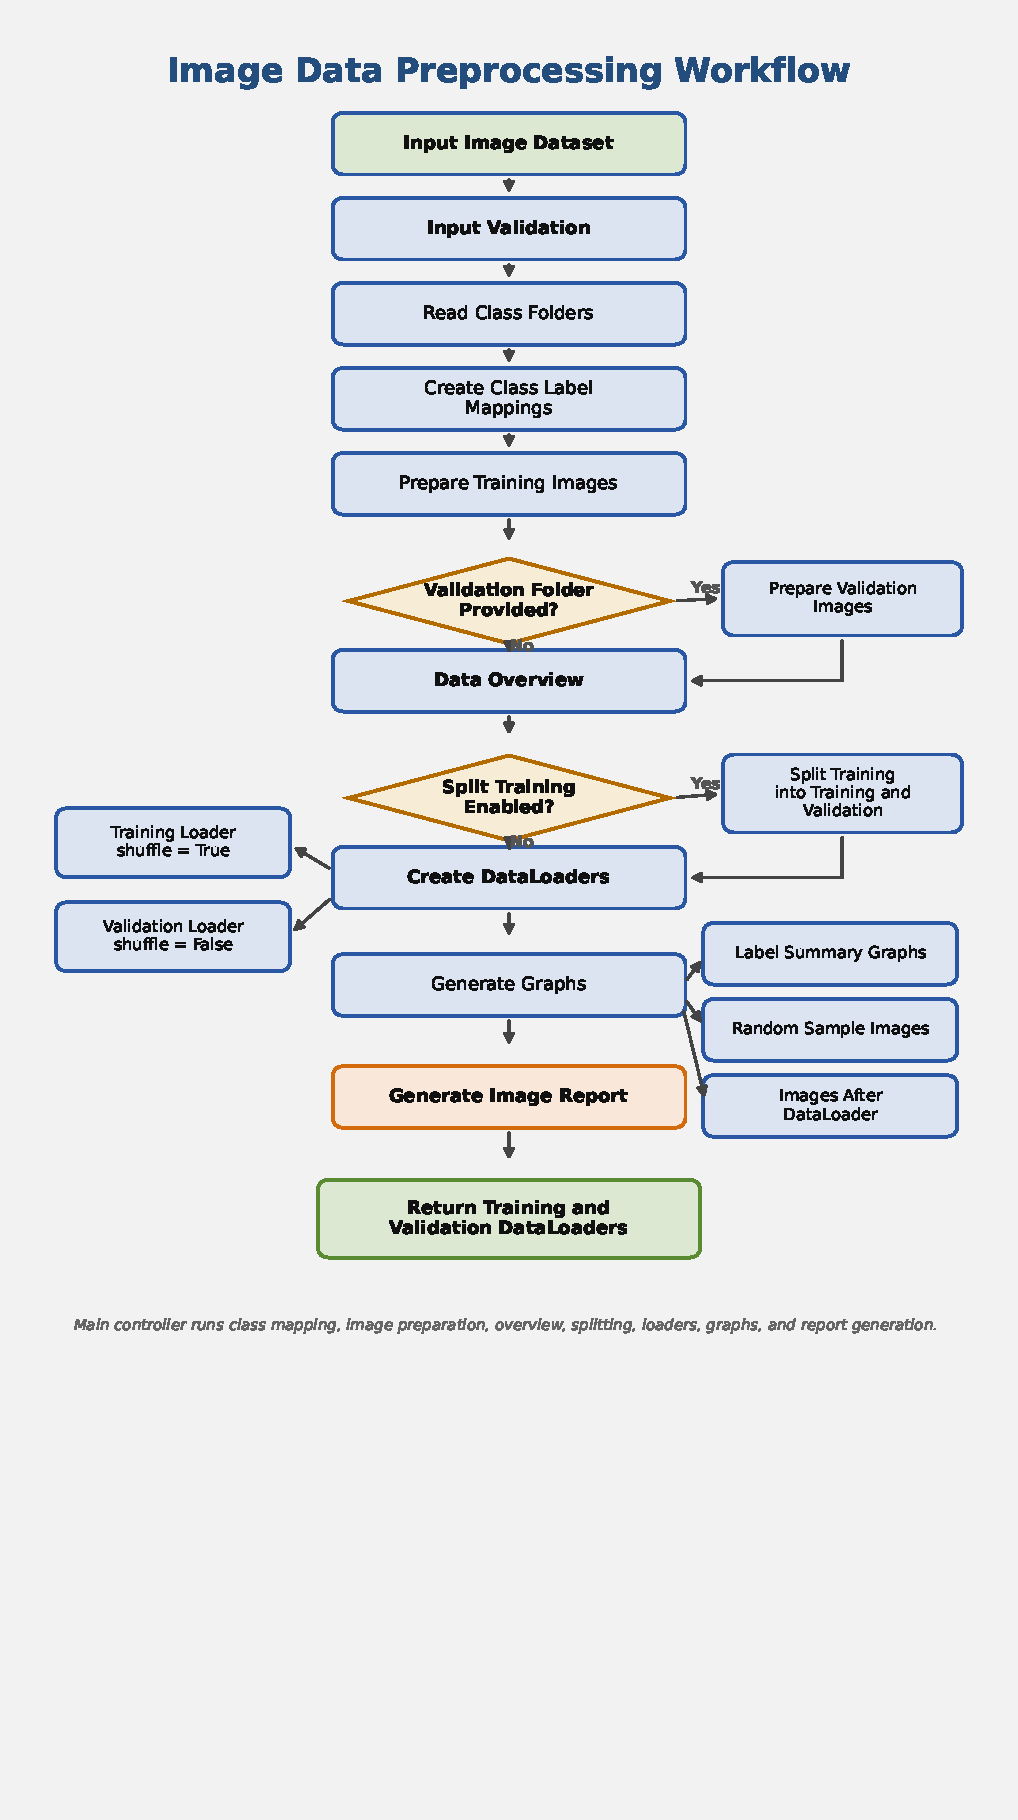
\includegraphics[width=\textwidth,trim=0mm 22mm 0mm 0mm,clip]{../imgs/image_workflow.pdf}
\caption{Image preprocessing workflow}
\label{fig:nesma-image-preprocessing-workflow}
\end{figure}
The image classification preprocessing class expects a folder structure where
each class has its own folder. It scans the folders, builds class-to-label and
label-to-class mappings, validates images, optionally splits the training
folder into training and validation sets, applies resizing and augmentation,
and returns PyTorch data loaders.

The validation folder is optional. If it is provided, its class folders must
match the training classes. If no validation folder is provided, the module can
split the training folder using the configured validation size. Invalid or
unreadable image files are not used for training, but they are recorded in the
report.

The image path saves:

\begin{itemize}[leftmargin=*]
  \item class-to-label mapping;
  \item label-to-class mapping;
  \item image size information; and
  \item report data about valid and invalid images.
\end{itemize}

The image report includes label summary graphs, random sample images from the
folders, and sample images after passing through the data loader. These graphs
are important because they show whether the class mapping, resizing, and
augmentation settings are working as expected.

The class mappings are created from the sorted training class names. This means
the same class name always receives the same numeric label as long as the class
folder names are the same. The mappings are saved in
\modulepath{class2label_mapping.pkl} and \modulepath{label2class_mapping.pkl}.
The selected image size is also saved in \modulepath{data_info.pkl}.

For each class folder, the module checks every image path using the image
validation utility. Valid images are stored with their numeric labels. Invalid
images are skipped, but their paths and labels are saved in the report data so
the user can know which files were removed. If no valid image exists, the
module raises an error instead of returning an empty loader.

The DataLoader construction is also different between training and validation.
The training loader uses shuffling and can apply augmentation. The validation
loader does not use augmentation and does not shuffle, because validation
should measure model behavior on stable data. The available augmentation
settings include horizontal flip, vertical flip, rotation, brightness change,
and contrast change, controlled by the probability and parameter values passed
to the constructor.

\begin{lstlisting}[style=algostyle,caption={Image training preprocessing flow from the implementation}]
Input: training image folder, optional validation folder
Output: training and validation DataLoaders

1:  Read class folders from the training directory
2:  Create class-to-label and label-to-class mappings
3:  Save mappings and image size information
4:  Validate image files and skip invalid images
5:  Build the data overview for the report
6:  Split training images if no validation folder is provided
7:  Create training dataset with resize and optional augmentation
8:  Create validation dataset without augmentation
9:  Build DataLoaders
10: Generate label, sample, and loader graphs
11: Generate the image preprocessing report
\end{lstlisting}

\subsection{Image Testing Flow}

The image testing class is used for new images after the training preprocessing
artifacts already exist. It loads the saved image size and class mapping,
validates the provided image paths, and creates a test dataset and DataLoader.
If class names are provided, each class name is converted to its saved numeric
label. If class names are not provided, the loader can still be used for
prediction-only mode.

Testing does not apply augmentation. It only applies the same resizing and
tensor conversion rules needed to make images compatible with the trained
model. Invalid images are returned separately, which is useful because the user
can see which inputs were ignored instead of silently losing files.

\subsection{Preprocessing Reports}

The Auto Preprocessing report belongs to the Auto Preprocessing module because
it explains what happened to the dataset during preprocessing. It is separate
from the Accelera pipeline report, which explains pipeline branches and metric
results.

For tabular data, \modulepath{TabularPreprocessingReport} receives the
\modulepath{report_data} dictionary collected during preprocessing. The report
contains:

\begin{itemize}[leftmargin=*]
  \item original and lowercased data previews;
  \item dataframe structure, numerical statistics, and categorical statistics;
  \item missing values, duplicate rows, and dataset shape;
  \item target-null handling and duplicate removal results;
  \item train-validation split sizes;
  \item dropped columns and the reason for each dropped column;
  \item EDA graphs generated for each feature column;
  \item preprocessing decision for every feature;
  \item processed samples of training and validation data; and
  \item feature-importance scores and selected features.
\end{itemize}

For text data, the same report class is reused in text mode. It shows the text
overview, text graph, target graph, cleaning and tokenization preview, TF-IDF
step, and encoded target samples. This helps show how raw
sentences became a sparse numerical matrix.

For image data, \modulepath{ImagePreprocessingReport} is used instead because
the input is folder-based. It shows class names, class-to-label mapping, number
of valid images, invalid image counts, invalid image paths, split information,
label summary graphs, random sample images, and samples after DataLoader
preprocessing.

This report is useful because preprocessing is usually a hidden part of a
machine-learning project. With the report, the user can see the important
changes instead of only receiving transformed arrays.


\section{Accelera Pipeline Reporting Module}



\subsection{Module Overview}

This chapter focuses only on the report classes related to
\modulepath{accelera_pipe}. These reports are different from the Auto
Preprocessing report. The Auto Preprocessing report explains data cleaning and
dataset transformation, while the pipeline report explains the executed
pipeline graph, branches, selected path, and metric results.

The pipeline reporting part has three main layers. \modulepath{ReportBase}
provides the shared HTML page structure. \modulepath{GraphPipelineReport}
groups and displays pipeline metric results. \modulepath{GraphReport} adds the
graph image, branch tables, and best-branch summary.

\subsection{Accelera Report Base}

\modulepath{ReportBase} defines shared HTML report behavior. It stores the
start and end HTML content, common styling, graph display helpers, and the
\modulepath{create_html_file} method that writes \modulepath{report.html}.
This class is important because different report classes can reuse the same
structure instead of each one writing a full HTML page from the beginning.

The base report also has a helper for showing saved graph images. It receives a
folder path and image names, checks whether the graph files exist, and adds the
images to the HTML content. This keeps graph display consistent for any report
that needs to include saved image files.

\subsection{Pipeline Metric Report}

\modulepath{GraphPipelineReport} is a pipeline reporting class, not the same as
the base Accelera report. It inherits from \modulepath{ReportBase}, but its job
is to format metric results produced by the pipeline execution. It receives a
list of metric result dictionaries. Each result contains the metric name, the
metric value, optional plotting function, labels, and headers.

The class groups results by metric name using \modulepath{handle_metric}. After
that, \modulepath{metric_display} chooses the suitable display wrapper based on
the result type:

\begin{itemize}[leftmargin=*]
  \item scalar numbers are displayed with \modulepath{DisplaySingleNumber};
  \item one-dimensional arrays are displayed with \modulepath{DisplayArraySingle};
  \item multi-dimensional arrays are displayed with \modulepath{DisplayMultiArray}
        or \modulepath{DisplayFigure};
  \item dictionaries are displayed with \modulepath{DisplayDict};
  \item strings are displayed with \modulepath{DisplayString}; and
  \item tuples are displayed with \modulepath{DisplayTupleNotCurve} or
        \modulepath{DisplayFigure}.
\end{itemize}

\subsection{Pipeline Graph Report}

\modulepath{GraphReport} is another pipeline report class. It extends
\modulepath{GraphPipelineReport}, but it adds graph-structure reporting. It
reads the serialized XML graph file, extracts nodes and edges, renders a
Graphviz image, finds branches through the graph, displays all branches, and
also shows the best branch based on nodes marked as selected in the final path.

The generated graph image labels each node using node id, node type, and node
name. Selected nodes are drawn in red, while the other nodes are drawn in blue.
Metric nodes are also collected so that the metric summary can be matched with
the graph branch where the metric was produced.

\begin{lstlisting}[style=algostyle,caption={Pipeline graph report generation flow}]
Input: XML graph path, metric results
Output: HTML pipeline report and graph image

1:  Parse the XML graph file
2:  Read nodes from XML layers
3:  Mark selected nodes and collect metric node ids
4:  Read edges and build graph connections
5:  Render the pipeline graph image with Graphviz
6:  Extract all branches until metric nodes are reached
7:  Group branches that share the same path
8:  Display all branches and the selected best branch
9:  Group metric results and format them by result type
10: Write report.html
\end{lstlisting}


\section{Benchmark Platform Module}



\subsection{Module Purpose}

The Benchmarking module provides a shared place for evaluating
machine-learning submissions. A benchmark creator defines the task, dataset
links, target column, and metric. Other users submit prediction files, and the
system calculates the score. This keeps comparison more fair because all users
are scored using the same target file and the same metric configuration.

The module is implemented in the \modulepath{benchmark} folder. It has a Node.js
and Express backend, MongoDB schemas using Mongoose, Python scripts for file
validation and scoring, and a React frontend for benchmark and leaderboard
screens.

\subsection{Functional Description}

When creating a benchmark, the user provides a title, description, problem
type, target column, dataset link, test dataset link, ground truth target link,
and evaluation metric. The module checks that the test dataset does not
include the target column and that the target file includes the required target
column. In the code, the target file is stored as
\modulepath{predictedColumnLink}, although it actually represents the true
target labels used for scoring submissions.

When submitting to a benchmark, the user provides a prediction file and a
repository link. The scoring process loads the target file and prediction file,
checks that they have the same number of rows, and computes the selected
metric. The submission is then saved and displayed in the leaderboard.

\subsection{Backend Architecture}

The backend server is started from \modulepath{benchmark/backend/server.js}. It
loads configuration, connects to MongoDB, enables CORS and JSON parsing, and
mounts the main routes:

\begin{itemize}[leftmargin=*]
  \item \modulepath{/metrics} for metric creation and listing;
  \item \modulepath{/benchmark} for benchmark creation and browsing; and
  \item \modulepath{/submission} for leaderboard submissions.
\end{itemize}

The backend uses schemas for benchmarks, metrics, and submissions. The route
files handle benchmark browsing and creation, metric browsing and creation,
and submission scoring. The Python scripts are called from the backend when
the system needs to validate uploaded links or calculate a submission score.

\subsection{Database Models}

The main benchmark data is stored in benchmark, metric, and submission
collections. The metric collection stores the display name, the scikit learn
metric function name, needed parameters, problem type, and whether higher or
lower values are better.

The benchmark collection stores the benchmark title, description, target
column, dataset link, test set link, target label link, problem type,
evaluation metric, metric parameters, creation date, and creator. The
submission collection stores benchmark id, submitter id, repository link,
prediction file link, submission date, and score. It also has an index on
benchmark id and score to support leaderboard access.

\subsection{Main Backend Components}

\begin{table}[!htbp]
\centering
\caption{Benchmarking module components}
\label{tab:benchmark components}
\begin{tabular}{p{0.28\textwidth}p{0.62\textwidth}}
\toprule
Component & Responsibility \\
\midrule
Benchmark management & Create, list, filter, view, and delete benchmark
tasks. \\
Metric management & Define metrics, problem type, parameters, and whether
higher or lower score is better. \\
Submission management & Store prediction submissions, repository links,
scores, submitter, and submission date. \\
Validation scripts & Check benchmark files and submission files before
scoring. \\
Scoring scripts & Compute the selected scikit learn metric on predictions and
ground truth. \\
Leaderboard interface & Display submissions ordered by the metric direction. \\
\bottomrule
\end{tabular}
\end{table}

\subsection{Benchmark Creation Flow}

The benchmark creation endpoint is implemented in
\modulepath{routes/benchmark.js}. The backend first normalizes the problem type
and checks that it is either classification or regression. It also checks that
the benchmark title is unique. Dataset and file links are validated, and Google
Drive file links are required for the test file and target file.

After link validation, the backend calls the Python validation script through
\modulepath{run_python}. The script downloads or retrieves the test and target
files, then checks two important rules:

\begin{enumerate}[leftmargin=*]
  \item the test dataset must not contain the target column; and
  \item the target file must contain the target column.
\end{enumerate}

The current validation script also checks that the target column is numeric.
If the validation succeeds, the benchmark is saved in MongoDB.

\begin{lstlisting}[style=algostyle,caption={Benchmark creation flow}]
Input: benchmark form data
Output: saved benchmark or validation error

1:  Receive benchmark creation request
2:  Validate problem type
3:  Check title uniqueness
4:  Validate dataset, test set, and target label links
5:  Run validate_user_links.py
6:  If the test file contains the target column, reject benchmark
7:  If the target file does not contain the target column, reject benchmark
8:  Save benchmark document in MongoDB
\end{lstlisting}

\subsection{Metric Management}

Metrics are managed through \modulepath{routes/metrics.js}. A metric is created
by providing a display name, scikit learn metric function name, problem type,
needed parameters, and \modulepath{whichBetter}. The
\modulepath{whichBetter} value must be either \modulepath{higher} or
\modulepath{lower}. This value is important because it controls leaderboard
sorting.

The system prevents duplicate metrics with the same name, problem type, and
scikit learn metric name. It also prevents deleting a metric if at least one
benchmark still uses it.

\subsection{Submission and Scoring Flow}

The submission endpoint is implemented in \modulepath{routes/submissions.js}.
The module prevents the same submitter from creating more than one submission
for the same benchmark. This is done by checking for an existing submission
with the same benchmark id and submitter id. If the submitter wants to change
the prediction file later, the update endpoint is used instead.

For each submission, the backend validates the repository link and prediction
file link. Then it calls \modulepath{get_score.py}. The Python script retrieves
the true labels and submitted predictions, checks that the files have the same
number of rows, checks that the prediction file contains the target column, and
then calls the selected metric from \modulepath{sklearn.metrics}.

\begin{lstlisting}[style=algostyle,caption={Submission scoring flow}]
Input: benchmark target file, submitted prediction file, metric name
Output: score or validation error

1:  Retrieve true target file
2:  Retrieve submitted prediction file
3:  Check that both files have the same number of rows
4:  Check that submitted file contains the target column
5:  Load metric function from sklearn.metrics
6:  Compute metric(true_target, predicted_target, metric_parameters)
7:  Return score to the backend as JSON
8:  Save submission with score
\end{lstlisting}

The scoring algorithm is kept in Python because the project already uses
Scikit learn metrics there. The backend sends the needed file links, target
column, metric name, and metric parameters. The Python script returns either a
score or an error message.

\subsection{Leaderboard Ordering}

Leaderboard ordering is handled by the submission route. When submissions are
requested for a benchmark, the backend reads the benchmark metric and checks
\modulepath{whichBetter}. If the metric is better when higher, submissions are
sorted by descending score. If the metric is better when lower, submissions are
sorted by ascending score. This lets the same module support metrics such as
accuracy and F1 score, where higher is better, and metrics such as mean
absolute error, where lower is better.

\subsection{Frontend Interface}

The frontend is implemented with React under
\modulepath{benchmark/frontend/src}. The relevant pages for benchmarking are:

\begin{itemize}[leftmargin=*]
  \item \modulepath{home.jsx}: entry page with links to benchmarks and metrics;
  \item \modulepath{benchmarks.jsx}: lists benchmarks and filters them by user
        or problem type;
  \item \modulepath{createBenchmark.jsx}: form for benchmark creation;
  \item \modulepath{metrics.jsx} and \modulepath{createMetric.jsx}: metric
        listing and metric creation;
  \item \modulepath{displayBenchmark.jsx}: shows benchmark details; and
  \item \modulepath{leaderBoard.jsx}: displays submissions and allows adding,
        updating, or deleting submissions when permitted.
\end{itemize}

\subsection{Benchmark Constraints}

The module has several important constraints:

\begin{itemize}[leftmargin=*]
  \item it currently supports classification and regression tasks;
  \item datasets and prediction files are provided as links;
  \item the test dataset must not contain the target column;
  \item the target file and prediction file must contain the selected target
        column;
  \item the target file and prediction file must have the same number of rows;
  \item metrics must map to valid scikit learn metric functions;
  \item benchmark creation and submission actions are protected by backend
        permission checks; and
  \item one user has only one active submission per benchmark, but the user can
        update it.
\end{itemize}


\chapter{System Testing and Verification}
\label{chap:testing-verification}

\section{Testing Setup}
The modules were tested using real datasets, saved preprocessing artifacts, generated reports, and benchmark workflow checks. The Auto Preprocessing results were evaluated by training machine learning models on the transformed outputs. Reporting was checked by generating HTML and graph outputs. Benchmarking was checked through benchmark creation, metric handling, submission validation, scoring, and leaderboard behavior.

\section{Testing Plan and Strategy}
The testing strategy focuses on verifying that each module works independently and that the generated outputs are usable by later steps. For preprocessing, the main check is that training artifacts are saved and can be reused during testing. For reporting, the main check is that report data is collected and rendered correctly. For benchmarking, the main check is that submissions are validated and scored using the same metric configuration.

\section{Module Testing}



\subsection{Auto Preprocessing Testing}

The Auto Preprocessing module was tested using unit tests and real datasets.
The tests check that outputs are generated correctly, report data is filled,
saved files exist, and test time preprocessing can reload training artifacts.

For tabular data, classification and regression datasets were processed and
then evaluated using machine learning models such as Random Forest. For text
data, the transformed TF IDF output was tested with a classifier. For image
data, the generated data loaders were tested with an image model. This was done
to check that the preprocessing output is usable for real training, not only
that the functions run.

\begin{table}[!htbp]
\centering
\small
\caption{Auto Preprocessing module testing results}
\label{tab:auto-preprocessing-module-results}
\begin{tabular}{p{0.40\textwidth}p{0.20\textwidth}p{0.24\textwidth}p{0.12\textwidth}}
\toprule
Dataset & Model & Metric & Result \\
\midrule
Startup founder burnout & Random Forest & Macro F1 score & 0.9999 \\
Healthy diet calorie intake & Random Forest & Macro F1 score & 1.0000 \\
Gaming addiction & Random Forest & Macro F1 score & 1.0000 \\
Student exam performance & Random Forest & Macro F1 score & 0.8573 \\
Heart & Random Forest & Macro F1 score & 0.7860 \\
Spine dataset & Random Forest & Macro F1 score & 0.7840 \\
Diabetes dataset & Random Forest & Macro F1 score & 0.9985 \\
Student placement synthetic & Random Forest & Macro F1 score & 0.9986 \\
Titanic dataset & Random Forest & Macro F1 score & 0.7906 \\
Customer purchase data & Random Forest & Macro F1 score & 0.9385 \\
Global AI jobs & Random Forest & R squared score & 0.9227 \\
Car price assignment & Random Forest & R squared score & 0.9562 \\
Housing & Random Forest & R squared score & 0.6037 \\
PetImages & ResNet & Accuracy & 0.9700 \\
DailyDialog & XGBClassifier & Macro F1 score & 0.9000 \\
TestReviews & XGBClassifier & Macro F1 score & 0.6080 \\
\bottomrule
\end{tabular}
\end{table}

These results show that the preprocessing output can be used by different
models after transformation. The tabular results were strong in many datasets,
especially the larger classification datasets and the car price regression
dataset. The lower scores on datasets such as  TestReviews show
that preprocessing alone does not solve every modeling problem. Some datasets
still need better features, model tuning, or more suitable models.

\subsection{Comparison with AutoCleanML}

The project also compares Accelera preprocessing with AutoCleanML on tabular
datasets. The comparison uses several classification and regression datasets
from Kaggle. For classification, the Macro F1 score is used. For regression,
the R squared score is used. The same split settings are used, with validation
size 20\% and random state 42.

After preprocessing, the output data was tested using four models: Logistic
Regression, Random Forest, Decision Tree, and KNN. The tables place the
AutoCleanML and Accelera scores beside each other for the same model, so the
comparison can be read directly.

\begin{table}[!htbp]
\centering
\small
\caption{Classification comparison using Logistic Regression and Random Forest}
\label{tab:classification-lr-rf-autoclean-accelera}
\begin{tabular}{p{0.38\textwidth}cccc}
\toprule
Dataset & \multicolumn{2}{c}{Logistic Regression} & \multicolumn{2}{c}{Random Forest} \\
\cmidrule(lr){2-3}\cmidrule(lr){4-5}
 & AutoCleanML & Accelera & AutoCleanML & Accelera \\
\midrule
Startup founder burnout & 1.0000 & 1.0000 & 0.9999 & 0.9999 \\
Healthy diet calorie intake & 0.9917 & 0.9890 & 1.0000 & 1.0000 \\
Gaming addiction & 0.8937 & 0.8937 & 0.9646 & 1.0000 \\
Student exam performance & 0.8667 & 0.8657 & 0.8579 & 0.8573 \\
Heart & 0.8019 & 0.8007 & 0.7689 & 0.7860 \\
Spine dataset & 0.8691 & 0.7943 & 0.8360 & 0.7840 \\
Diabetes dataset & 0.9995 & 0.9985 & 0.9996 & 0.9985 \\
Student placement synthetic & 0.5657 & 0.5879 & 0.6241 & 0.9986 \\
Titanic dataset & 0.7734 & 0.7864 & 0.7906 & 0.7906 \\
Customer purchase data & 0.8484 & 0.8375 & 0.9386 & 0.9385 \\
\bottomrule
\end{tabular}
\end{table}

\begin{table}[!htbp]
\centering
\small
\caption{Classification comparison using Decision Tree and KNN}
\label{tab:classification-dt-knn-autoclean-accelera}
\begin{tabular}{p{0.38\textwidth}cccc}
\toprule
Dataset & \multicolumn{2}{c}{Decision Tree} & \multicolumn{2}{c}{KNN} \\
\cmidrule(lr){2-3}\cmidrule(lr){4-5}
 & AutoCleanML & Accelera & AutoCleanML & Accelera \\
\midrule
Startup founder burnout & 1.0000 & 1.0000 & 0.9824 & 0.9881 \\
Healthy diet calorie intake & 1.0000 & 1.0000 & 0.9379 & 0.9184 \\
Gaming addiction & 1.0000 & 1.0000 & 0.6905 & 0.8512 \\
Student exam performance & 0.7987 & 0.8063 & 0.8423 & 0.8338 \\
Heart & 0.7213 & 0.7704 & 0.7689 & 0.7860 \\
Spine dataset & 0.7686 & 0.7632 & 0.8239 & 0.8042 \\
Diabetes dataset & 0.9995 & 0.9972 & 0.9925 & 0.9980 \\
Student placement synthetic & 0.5827 & 0.9968 & 0.5995 & 0.8348 \\
Titanic dataset & 0.6979 & 0.7877 & 0.7203 & 0.7562 \\
Customer purchase data & 0.8486 & 0.8449 & 0.8544 & 0.8806 \\
\bottomrule
\end{tabular}
\end{table}

\begin{table}[!htbp]
\centering
\small
\caption{Regression comparison using Linear Regression and Random Forest}
\label{tab:regression-lr-rf-autoclean-accelera}
\begin{tabular}{p{0.38\textwidth}cccc}
\toprule
Dataset & \multicolumn{2}{c}{Linear Regression} & \multicolumn{2}{c}{Random Forest} \\
\cmidrule(lr){2-3}\cmidrule(lr){4-5}
 & AutoCleanML & Accelera & AutoCleanML & Accelera \\
\midrule
Global AI jobs & 0.9022 & 0.7498 & 0.9288 & 0.9227 \\
Car price assignment & 0.8886 & 0.8943 & 0.9535 & 0.9562 \\
Housing & 0.6506 & 0.6482 & 0.6087 & 0.6037 \\
\bottomrule
\end{tabular}
\end{table}

\begin{table}[!htbp]
\centering
\small
\caption{Regression comparison using Decision Tree and KNN}
\label{tab:regression-dt-knn-autoclean-accelera}
\begin{tabular}{p{0.38\textwidth}cccc}
\toprule
Dataset & \multicolumn{2}{c}{Decision Tree} & \multicolumn{2}{c}{KNN} \\
\cmidrule(lr){2-3}\cmidrule(lr){4-5}
 & AutoCleanML & Accelera & AutoCleanML & Accelera \\
\midrule
Global AI jobs & 0.8640 & 0.8412 & 0.7586 & 0.7510 \\
Car price assignment & 0.9269 & 0.8825 & 0.7905 & 0.7478 \\
Housing & 0.3819 & 0.3634 & 0.5312 & 0.5336 \\
\bottomrule
\end{tabular}
\end{table}

From these results, Accelera preprocessing is generally close to AutoCleanML,
but it is not better in every case. In several classification datasets the two
tools give almost the same score, such as startup founder burnout, healthy diet,
diabetes, Titanic, and customer purchase data. Accelera is clearly better in
some cases, especially student placement synthetic with Random Forest, Decision
Tree, and KNN, and gaming addiction with Random Forest and KNN. AutoCleanML is
better in other cases, such as spine dataset and the linear regression result
for global AI jobs. So, the comparison shows that Accelera preprocessing gives
valid and competitive results, but the best result still depends on the dataset
and the model used after preprocessing.

\subsection{Pipeline Reporting Module Testing}

The graph report is exercised through examples that build branch-based
workflows, serialize the graph to XML, and run \modulepath{GraphReport}. The
expected result is a \modulepath{report.html} file and a graph image showing
the serialized graph structure. The report also checks that metrics are displayed
according to their result type.

\subsection{Benchmarking Module Testing}

The Benchmarking module was tested manually by submitting different model
results and checking whether the submitted results were saved and displayed in
the leaderboard. The main checked behavior was that the module receives a
submission, stores the dataset name, metric name, and score, and orders the
leaderboard correctly.

\subsection{Testing Datasets}

\begin{table}[!htbp]
\centering
\caption{Examples of datasets used in Auto Preprocessing testing}
\label{tab:testing-datasets}
\begin{tabular}{p{0.45\textwidth}p{0.20\textwidth}p{0.25\textwidth}}
\toprule
Dataset & Data type & Problem type \\
\midrule
\modulepath{startup_founder_burnout_2026} & Tabular & Classification \\
\modulepath{healthy_diet_calorie_intake} & Tabular & Classification \\
\modulepath{ai_student} & Tabular & Classification \\
\modulepath{Titanic-Dataset} & Tabular & Classification \\
\modulepath{global_ai_jobs} & Tabular & Regression \\
\modulepath{CarPrice_Assignment} & Tabular & Regression \\
\modulepath{Housing} & Tabular & Regression \\
\modulepath{PetImages} & Image & Classification \\
\modulepath{DailyDialog} & Text & Classification \\
\modulepath{TestReviews} & Text & Classification \\
\bottomrule
\end{tabular}
\end{table}


\chapter{Conclusions and Future Work}
\label{chap:conclusions-future-work}

\section{Faced Challenges}
The main challenges were keeping preprocessing consistent between training and testing, supporting different dataset types inside one module, generating useful reports without mixing report logic with preprocessing logic, and designing a benchmark workflow that evaluates all submissions fairly.

\section{Gained Experience}
This work provided practical experience in automated data preprocessing, report generation, feature engineering, metric handling, backend workflow design, and testing machine learning support modules using real datasets.

\section{Conclusions}



This report documented the Auto Preprocessing module, the Reporting module,
and the Benchmarking module in Accelera. The Auto Preprocessing
module automates repeated preparation steps for tabular, text, and image data
and saves artifacts for consistent testing. The Reporting module uses HTML
pages, tables, saved figures, and metric display wrappers to explain outputs.
The Benchmarking module provides a shared
evaluation workflow for comparing prediction submissions using the same metric
and ground truth.

Together, these parts support a more complete data-science workflow. The user
can prepare data, inspect generated reports, and compare final predictions in a
benchmark. The implementation still has limitations, but it gives a clear base
for future development and evaluation.


\section{Future Work}



\subsection{Design Advantages}

The main advantage of Auto Preprocessing is consistency. The same fitted
objects used during training are saved and loaded during testing. This reduces
the chance of data leakage and mismatched transformations. Another advantage is
that the module supports more than one data type, so the same project can
prepare tabular, text, and image datasets.

The main advantage of the Reporting module is explainability. The user can see
data summaries, generated visualizations, preprocessing decisions, graph
structure when available, and metric results in one place.

The Benchmarking module helps make comparison fairer because all submissions
are evaluated using the same ground truth and metric configuration.

\subsection{Current Limitations}

There are also limitations:

\begin{itemize}[leftmargin=*]
  \item the preprocessing rules are fixed heuristics and may not be optimal for
        every dataset;
  \item the tabular preprocessing path assumes ordinary structured data and may
        need extensions for time-series or special domain data;
  \item text preprocessing uses classical TF-IDF, not transformer-based
        language models;
  \item image preprocessing prepares data loaders but does not automatically
        choose the best neural network architecture;
  \item graph report generation depends on graph serialization before
        report execution;
  \item benchmark files are provided through links, so file availability
        depends on external storage; and
  \item the benchmark testing described in the current report is mainly manual.
\end{itemize}

\subsection{Possible Improvements}

Future improvements can include adaptive preprocessing based on the model type,
better handling of imbalanced datasets, more advanced text preprocessing,
server-side benchmark file storage, stronger automated tests for the
Benchmarking module, and more polished report templates. The graph report can also be
extended to include execution time and memory information for each branch.


\appendix
\chapter{User Guide}
\label{chap:user-guide}



This chapter gives simple examples for calling the main classes from the code.
The examples are small, but they show the normal constructor calls and the main
method used to start preprocessing or report generation.

\section{Using Tabular Auto Preprocessing}

For tabular data, the user loads the dataset as a Pandas DataFrame, chooses the
target column, chooses the problem type, and gives an output folder. The output
folder stores the fitted preprocessing objects and the report.

\begin{lstlisting}[style=code,caption={Calling tabular training preprocessing}]
import pandas as pd
from accelera.src.auto_preprocessing.core.classical_training_preprocessing import (
    ClassicalTrainingPreprocessing,
)

df = pd.read_csv("dataset.csv")

preprocessor = ClassicalTrainingPreprocessing(
    df=df,
    target_col="target",
    problem_type="classification",
    folder_path="outputs/tabular_run",
    val_size=0.2,
    random_state=42,
    is_report=True,
)

X_train, y_train, X_val, y_val = preprocessor.common_preprocessing()
\end{lstlisting}

For regression, the main change is the problem type and target column.

\begin{lstlisting}[style=code,caption={Calling tabular regression preprocessing}]
preprocessor = ClassicalTrainingPreprocessing(
    df=df,
    target_col="price",
    problem_type="regression",
    folder_path="outputs/regression_run",
)
\end{lstlisting}

For test data, the user should pass the same folder path. This makes the test
data use the saved training transformers instead of fitting new transformers.

\begin{lstlisting}[style=code,caption={Calling tabular testing preprocessing}]
import pandas as pd
from accelera.src.auto_preprocessing.core.classical_testing_preprocessing import (
    ClassicalTestingPreprocessing,
)

test_df = pd.read_csv("test.csv")

test_preprocessor = ClassicalTestingPreprocessing(
    df=test_df,
    folder_path="outputs/tabular_run",
)

X_test, y_test = test_preprocessor.common_preprocessing()
\end{lstlisting}

\section{Using Text Auto Preprocessing}

For text data, the user provides the text column and target column. The module
cleans the text, applies TF-IDF, encodes the labels, and saves the needed
objects.

\begin{lstlisting}[style=code,caption={Calling text training preprocessing}]
import pandas as pd
from accelera.src.auto_preprocessing.core.text_training_preprocessing import (
    TextTrainingPreprocessing,
)

df = pd.read_csv("reviews.csv")

text_preprocessor = TextTrainingPreprocessing(
    df=df,
    target_col="label",
    text_col="review",
    folder_path="outputs/text_run",
    tfidf_max_features=500,
    is_report=True,
)

X_train, y_train, X_val, y_val = text_preprocessor.common_preprocessing()
\end{lstlisting}

For testing text data, the user again passes the same folder path. If the test
data does not contain the target column, the class returns the transformed text
features and \modulepath{None} for labels.

\begin{lstlisting}[style=code,caption={Calling text testing preprocessing}]
from accelera.src.auto_preprocessing.core.text_testing_preprocesing import (
    TextTestingPreprocessing,
)

test_text = pd.read_csv("reviews_test.csv")

text_test_preprocessor = TextTestingPreprocessing(
    df=test_text,
    folder_path="outputs/text_run",
)

X_test, y_test = text_test_preprocessor.common_preprocessing()
\end{lstlisting}

\section{Using Image Auto Preprocessing}

For image preprocessing, the dataset should be arranged as class folders. For
example:

\begin{verbatim}
Training/
  Cats/
  Dogs/
\end{verbatim}

The user passes the training folder and output folder. If there is no separate
validation folder, the module can split the training folder.

\begin{lstlisting}[style=code,caption={Calling image training preprocessing}]
from accelera.src.auto_preprocessing.core.classification_image_training_preprocessing import (
    ClassificationImageTrainingPreprocessing,
)

image_preprocessor = ClassificationImageTrainingPreprocessing(
    training_folder_images="data/PetImages/Training",
    folder_path="outputs/image_run",
    split_training=True,
    val_size=0.2,
    images_size=(224, 224),
    batch_size=16,
    augment=True,
)

train_loader, val_loader = image_preprocessor.common_preprocessing()
\end{lstlisting}

For image testing, the user provides a list of image paths. Class names are
optional, but if they are provided, they must match the saved training classes.

\begin{lstlisting}[style=code,caption={Calling image testing preprocessing}]
from accelera.src.auto_preprocessing.core.classification_image_testing_preprocessing import (
    ClassificationImageTestingPreprocessing,
)

image_paths = ["test/cat1.jpg", "test/dog1.jpg"]
class_names = ["Cats", "Dogs"]

image_test_preprocessor = ClassificationImageTestingPreprocessing(
    image_paths=image_paths,
    image_class_names=class_names,
    folder_path="outputs/image_run",
    batch_size=4,
)

test_loader, invalid_images = image_test_preprocessor.common_preprocessing()
\end{lstlisting}

\section{Reading Auto Preprocessing Reports}

After running preprocessing with \modulepath{is_report=True}, the user opens
the generated \modulepath{report.html} file from the output folder. The report
shows the dataset overview, missing values, duplicate rows, dropped columns,
graphs, preprocessing decisions, selected features, and processed data samples.

\section{Using Pipeline Reports}

To generate a pipeline report, the pipeline graph should be serialized first.
Then the user passes the XML graph path, output folder, and metric results to
\modulepath{GraphReport}.

\begin{lstlisting}[style=code,caption={Calling the pipeline graph report}]
from accelera.src.accelera_pipe.wrappers.graph_report import GraphReport

report = GraphReport(
    folderpath="outputs/pipeline_report",
    xmlpath="outputs/pipeline_graph.xml",
    results=metric_results,
)

report.execute()
\end{lstlisting}

The output is a \modulepath{report.html} file. It contains the graph image,
branch tables, selected branch, and metric summary.

\section{Using the Benchmark Platform}

The benchmark platform is used from the web interface. The benchmark creator
enters the title, problem type, target column, dataset link, test-set link,
target-label link, and evaluation metric. A user submits a prediction file link
and repository link. The backend calls the Python scoring script, saves the
score, and displays the result in the leaderboard.

The prediction file must contain the target column expected by the benchmark.
Also, the number of rows in the prediction file must match the number of rows
in the target-label file.

\end{document}
